\Chapter{Téma elméleti kifejtése}
\label{Chap:tema}

\Section{Mobil alkalmazások}
Napjainkban rengeteg különböző kerékpáros alkalmazás érhető el amik más más területre fókuszálnak. A következő pontokban ezekre láthatunk néhány példát az egyszerű mérnöki alapú számítástól az útvonalak nyomon követésén keresztül a fejlett, összetett tervező rendszerekig. Látható hogy a felhasználók körében nagy népszerűségnek örvend a különböző alkalmazások közösségi funkciói ahol lehetőség van az ismerősök megtalálására, útvonalak megosztására.  

\SubSection{Bike calculator}
A "Bike Calculator" \cite{bikecalculator} weboldal és mobil alkalmazás biciklis becsléseket kínál a felhasználói számára, teljesen mérnöki szempontból. A modell figyelembe veszi a sebesség, erőkifejtés, szélellenállás, gravitáció és egyéb tényezők összefüggését azonban egy általános eredményt ad, nincs lehetőség a felhasználó egyéni teljesítményének figyelembe vételére. Ezzel együtt is egy érdekes megoldás ami rengeteg paramétere révén jól skálázható.

\SubSection{Strava}
A Strava \cite{strava} az egyik legelterjedtebb alkalmazás a sporttevékenységüket nyomon követni kívánók körében, széles funkcionalitással és hatalmas felhasználói bázissal. Lehetőséget nyújt többek között biciklizés, futás, úszás, hegymászás és rengeteg egyéb sportág eredményeinek rögzítésére és korlátozott szintű tervezésére. A tevékenység során rögzített adatokból alapvető statisztikákat készít a felhasználók számára, mint a sebesség és a tengerszint feletti magasság változása valamint a sportoló pulzusának mozgása. Népszerűsíti a Strava-t hogy lehetőséget kínál az ismerősök megtalálására és az útvonalak, tevékenységek megosztására valamint kommentek és "kudo"-k egyfajta elismerés, tetszés nyilvánítás adására. Érdekes funkciói közé tartozik a szegmensek, rövid útvonal szakaszok kezelése ahol a felhasználóknak lehetőségük van rövid távon versenyezni, előrébb kerülni a szegmenst teljesítők listáján valamint számon tartani a saját rekordjaikat. 

A Strava tervezője, jövővel kapcsolatban segítő funkciója egy útvonal tervezőben merül ki,ami segíti a felhasználókat a legnépszerűbb út megtalálásában A és B pont között, térképpel és részletes navigációs leírásokkal. Az útvonal kijelölésénél az alapvető adatokon kívül egy becslést is kapunk a várható időre nézve. A várható idő számolása a bejelentkezett felhasználó legutóbbi 4 heti teljesítménye alapján történik. Előrelépés hogy egyáltalán figyelembe veszi a felhasználó eddigi útvonalait azonban ennek a módszernek is vannak hiányosságai így csak egy közepes kiindulási alapot ad. Alapvető gond ezzel a becsléssel hogy az útvonalak rögzítésénél a felhasználó hiába állítja be az út típusát (verseny, edzés, ingázás stb.) a Strava számítás során ezeket nem veszi figyelembe, így könnyen előfordulhat hogy a felhasználó kiugróan pontatlan, akár használhatatlan eredményt kap. Például az előző hetekben a saját határait feszegetve versenyre készült, most viszont szeretne egy nyugodt családi biciklizésre elindulni - ekkor nyilván nem fog rekordokat dönteni és a Strava által számolt várható idő semmilyen tényleges információval nem fog szolgálni számára.


\SubSection{Endomondo}
Az Endomondo \cite{endomondo} webes és mobil alkalmazás sporttevékenység nyomon követését hivatott megkönnyíteni a felhasználói számára. Rengeteg különböző sportágat megkülönböztet, ezekről külön statisztikákat készít valamint egyéni célokat lehet ezekre vonatkozóan beállítani. Az egyes sportágakat GPS alapú jelkövetés segítségével lehet nyomon követni, illetve kézzel is létrehozhatóak új tevékenységek, továbbá lehetőség van különböző alkalmazásokból vagy fájlból importálni korábban teljesített útvonalakat. Az alkalmazás megvalósít közösségi funkciókat is, a felhasználóknak lehetőségük van megkeresni az ismerőseiket akikkel később megoszthatják legújabb sporttevékenységüket valamint versenghetnek egymással a közösen felállított célok eléréséért. Az Endomondo érdekes adaléka hogy mozgás közben audió visszajelzést biztosít a felhasználók számára az addigi teljesítményükről, így a felhasználók sportolás közben is pontos információval rendelkezhetnek anélkül hogy az alkalmazást futtató eszközüket kellene figyelniük.


\SubSection{Best Bike Split}
A Best Bike Split \cite{bestbikesplit} egy rendkívül összetett rendszer amely elsősorban versenyzők számára kínál széles funkcionalitást. Alapköve a versenytáv megtételének optimalizálása melynek keretei között személyre szabott, szakaszokra bontott tervet állít fel a felhasználó számára annak érdekében hogy a tervezett távot a lehető legjobb idő alatt teljesítse. Ez a terv alapul veszi a felhasználó biciklijének és felszerelésének a tulajdonságait (kerekek típusa, bicikli súlya, sisak kialakítása stb.) a preferált versenyzési módot (elhelyezkedés a verseny során, sík terep illetve emelkedő esetén) valamint már teljesített edzést, versenyeket és természetesen a teljesítendő verseny paramétereit. Prémium előfizetés használata során a kalkulációt befolyásolja a várható időjárás is. A rendszer használható tetszőleges útvonalakra azonban az átlag kerékpáros számára szükségtelenül bonyolult, összetett így elsősorban versenyzők számára hasznos.

\SubSection{Összefoglalás és célkitűzés}
Több tucatnyi hasonló alkalmazás létezik, webes felülettel illetve Android és iOS lefedéssel hiszen a kerékpározás fellendülőben van napjainkban, így egyre több alkalmazás készül a felhasználói igények kielégítésére mind versenyzők mind pedig hétköznapi felhasználók számára akiknek a biciklizés inkább közlekedési mint sport eszköz. Ezen alkalmazások felsorolása vagy részletezése nem célja ennek a szakdolgozatnak, azonban néhány példa alapján is könnyen meghatározhatóak általános csoportok amelyekbe a létező megoldások besorolhatóak.


\subsubsection{Útvonal rögzítés} 
A legalapvetőbb funkció amire különböző megoldások léteznek. A legegyszerűbb eszközök esetén például csak az aktuális sebesség és a távolság kerül megállapításra egy, a kerékre rögzíthető érzékelőnek a segítségével. Az érzékelő használatával számolni lehet hogy a kerék hányszor fordul körbe adott időablakon belül, ennek és a kerék méretének felhasználásával könnyen megállapítható a pillanatnyi sebesség illetve az útvonal kezdete óta megtett távolság. Azonban a növekvő igényekhez igazodva ma már lényegesen elterjedtebbek a GPS alapú mobil alkalmazások amik a pillanatnyi sebességen és távolságon kívül pontosan tudják rögzíteni az út egyéb paramétereit is mint pl.: kezdő és végpont koordinátái, mozgással töltött idő, megtett emelkedő, legalacsonyabb és legmagasabb pont, átlag sebesség, maximum sebesség. Ezek a jellemzők lényegesen pontosabb leírást adnak egy-egy útvonalról, tárolásukkal könnyen nyomon követhető a személyes fejlődés, kitűzhetőek heti, havi, éves célok. Az útvonal paramétereinek nyomon követése, struktúrája és tárolása megvalósításonként változó, azonban a cél mindig ugyanaz: minél több jellemző meghatározása a lehető legrészletesebb módon.

\subsubsection{Közösségi funkciók} 
A kerékpáros útvonalakat nyomon követő mobil alkalmazások elterjedésével egy új tendencia jelent meg; egyre többször figyelhető meg valamilyen jellegű közösségi funkció megvalósítása az alkalmazáson belül, amik nagy népszerűségnek örvendenek az alkalmazást használók körében. Ezen funkciók nagyban különbözhetnek, általánosságban lehetőség van az alkalmazást használó ismerősök megtalálására, megtett útvonalak megosztására illetve valamilyen formában tetszésnyilvánítás / elismerés adására. Ezeken kívül általában megjelenik valamilyen ösztönzés, lelkesítés ami segíthet a teljesítmény javításában, a kitűzött célok elérésében. A Strava esetében ez a szegmensek formájában jelenik meg, amik lényegében rövid, maximum néhány száz méteres útvonalak, általában valamilyen szempontból nehezebb szakaszok (pl.: emelkedő). Ezen szegmensek teljesítésével a felhasználó automatikusan felkerül több rangsorra is (globális, adott évre vonatkozó, nem és korcsoport alapján lebontott) ahol lehetősége van ismerősökkel és ismeretlenekkel vetélkedni ezzel felébresztve a versenyszellemet. 

\subsubsection{Tervezés, becslés} 
A kerékpáros alkalmazások fejlődésének következő lépcsőfoka az útvonalak tervezése és a teljesítmény becslése. Útvonalak tervezésére kevésbé kerékpár specifikus alkalmazások is lehetőség adnak mint például a Google Térkép de sok, kifejezetten kerékpárosoknak készült alkalmazásban is léteznek megvalósítások. A tervezés különböző szempontok alapján történhet: egyik fontos szempont a távolság (ez a legfontosabb amennyiben a cél az út minél gyorsabb megtétele A és B pont között), egy másik pedig a népszerűség szóval foglalható össze. Az utóbbi főleg akkor fontos ha a kerékpározásra nem közlekedés szerűen tekintünk hanem inkább mint sport, kikapcsolódás hiszen ilyenkor előrébb kerül a jogos felhasználói igény az olyan útvonalakra ahol szép környezetben, lehetőség szerint autós és gyalogos forgalomtól zavartalanul lehet kerékpározni. Az útvonalak tervezéséhez szorosan kapcsolódik a teljesítmény, a várható idő meghatározása ami koránt sem egyszerű feladat. Ennek legalapvetőbb megoldása a Bike calculator által is megvalósított mérnöki, fizikai modell, ahol a teljesítmény tisztán a felszerelés és a megtenni kívánt út paraméterei alapján kerül kiszámításra


\subsubsection{Tervezés, becslés - egyéni teljesítmény alapján} 
Az útvonal tervezés és a várható teljesítmény becslésének továbbfejlesztésének, pontosításának alapjául az eddig megtett útvonalak és az elért eredmények szolgálhatnának, ez azonban egy olyan terület ahol még nem sok megoldás született. Ide sorolható a Strava által fejlesztett útvonal tervező, ahol a várható idő becsléséhez alapul veszi a bejelentkezett felhasználó elmúlt 4 heti teljesítményét, és míg ez egy jó kezdeményezés a valóságban nem mindig szolgál pontosabb információval mint egy egyszerű, fizikai összefüggéseken alapuló általános modell. Megnehezíti a pontos becslések készítését hogy egy adott felhasználó sokszor kevés adattal rendelkezik amelyek nem elég változatosak egy új útvonal esetén várható teljesítmény megbecsléséhez.\\[12pt]

\noindent
A fenti csoportok összefoglalása a vizsgált alkalmazásokra:
\begin{table}[!h]
	\resizebox{\textwidth}{!}{%
	\begin{tabular}{c|c|c|c|c|}
		\cline{2-5}
		\multicolumn{1}{l|}{} & 
		\multicolumn{1}{l|}{\textbf{Bike calculator}} & 
		\multicolumn{1}{l|}{\textbf{Strava}} & 
		\multicolumn{1}{l|}{\textbf{Endomondo}} & 
		\multicolumn{1}{l|}{\textbf{Best Bike Split}} \\ \hline
		
		\multicolumn{1}{|c|}{
			\begin{tabular}
				[c]{@{}c@{}}Útvonal \\ rögzítés
		\end{tabular}} & 
		{\color[HTML]{FE0000} $\boldsymbol{\times}$} & {\color[HTML]{009901} \textbf{\checkmark}} & {\color[HTML]{009901} \textbf{\checkmark}} & {\color[HTML]{009901} \textbf{\checkmark}}             \\ \hline
		\multicolumn{1}{|l|}{
			\begin{tabular}
				[c]{@{}l@{}}Közösségi \\ funkciók
		\end{tabular}} &
		{\color[HTML]{FE0000} \textbf{$\boldsymbol{\times}$}} & {\color[HTML]{009901} \textbf{\checkmark}} & {\color[HTML]{009901} \textbf{\checkmark}} & {\color[HTML]{FE0000} $\boldsymbol{\times}$}         \\ \hline
		
		\multicolumn{1}{|c|}{
			\begin{tabular}
				[c]{@{}c@{}}Tervezés\\ (általános)
		\end{tabular}} & 
		{\color[HTML]{009901} \textbf{\checkmark}} & {\color[HTML]{009901} \textbf{\checkmark}} & {\color[HTML]{009901} \textbf{\checkmark}} & {\color[HTML]{009901} \textbf{\checkmark}}     \\ \hline
		
		\multicolumn{1}{|c|}{
			\begin{tabular}
				[c]{@{}c@{}}Tervezés\\ (egyéni)
		\end{tabular}}   &
		{\color[HTML]{FE0000} $\boldsymbol{\times}$} & {\color[HTML]{009901} \textbf{\checkmark}} & {\color[HTML]{FE0000} $\boldsymbol{\times}$} & {\color[HTML]{009901} \textbf{\checkmark}}             \\ \hline
	\end{tabular}
	}
\end{table}


\subsubsection{Célkitűzés}
Ezen 4 fő csoport közül az első három által meghatározott problémákra, igényekre mára már rengeteg, változatos módon megvalósított megoldás létezik, így ezeknek a tárgyalásától a továbbiakban eltekintünk. Azonban az utolsó probléma, a felhasználó egyéni teljesítményének figyelembe vétele egy nyitott terület, ahova nem sokan merészkedtek még, így a szakdolgozat során összehasonlításra kerülő gépi tanulási algoritmusok célja sportolói teljesítmény becslése. A teljesítményt természetesen nagy mértékben befolyásolja a kerékpáros felszerelések minősége és állapota, az útvonal terep és időjárás viszonyai azonban az egyén általános és pillanatnyi fizikai és szellemi állapota (kimerültség, kedvtelenség stb.) nem elhanyagolható tényező. Az átlagos értelemben vett teljesítmény több részre bontható le a kerékpározás kapcsán, melyek a szakdolgozat során külön kerülnek megválaszolásra.


%%%%%%%%%%%%%%%%%%%%%%%%%%%%%%%%%%%%%%%%%%%%

\Section{Megválaszolandó kérdések}
A sportteljesítmény becslése nehéz feladat, mivel egyénenként nagyon eltérő lehet, valamint az út nyers adatain kívül (távolság, emelkedő, időjárás) a egyén pillanatnyi fizikai és szellemi állapota is nagyban befolyásolja (álmosság, kimerültség, kedvtelenség stb.). Ezért el kell dönteni hogy egy általános modell megépítése a cél, ami esetleg életkor, nem, edzettségi szint szerint finomhangolható azonban kisebb pontossággal rendelkezik, vagy személyre szabott, pontos becsléseket kell elérni ahol viszont a gépi tanulás során nehézséget okozhat a kis méretű adathalmaz, hiszen kevesen rendelkeznek akár csak néhány száz rögzített úttal, míg a megfelelő pontossághoz ehhez nagyságrendekkel több adatra van szüksége az egyes algoritmusoknak




\SubSection{Nehézségi osztályok meghatározása}
A Strava-ról gyűjtött utak sok adatot tartalmaznak azonban nincsenek kategorizálva, így cél az eddig megtett utakat nehézség alapján több osztályba sorolni, azonban ennek megvalósítása kérdéses. Mivel a helyes label-ek hiányoznak klaszterezési módszereket kell használni. Várhatóan az egyén adatai alapján és a összes összegyűjtött adat alapján készült osztályok különbözőek lesznek, hiszen más útvonalakat tettek meg, eltérő eredményekkel.

Egy általános modell elkészítése az elsődleges feladat, mivel az adatok sokszínűsége és mennyisége miatt jobb kiindulópontot jelent. Amennyiben egy adott felhasználó megfelelően sok és sokféle útvonal adattal rendelkezik akkor érdemes lehet egyéni, személyre szabott nehézségi csoportok kialakításával is foglalkozni.

%\SubSection{Nehézség meghatározása - új útvonalra}
%A már megtett útvonalak osztályozása után a következő lépés az új, megtenni kívánt útvonalak nehézségének meghatározása. Ez megvalósítható egyrészt a már betanított klaszterezési algoritmusok felhasználásával, másrészt a klaszterezés által meghatározott osztályok label-jeit felhasználva valamilyen osztályozással. 


%Időpont is érdekes lehet (reggeli / esti között van e különbség)
\SubSection{Időtartam becslés}

Az egyik legalapvetőbb feladat a várható idő meghatározása, hiszen ez az egyik legmeghatározóbb pontja a kerékpározásnak - mennyi időbe fog telni mire megtesz valaki adott távolságot? Ennek a kérdésnek a megválaszolására alapvetően a különböző regressziók alkalmasak, amik az út paraméterei alapján folytonos értéket adnak vissza. Azonban ez a pont kicsit bonyolultabb mint amilyennek tűnik, mivel alapvetően kétféle időtartamot különböztetünk meg: a mozgási és a tényleges időtartamot. Az első jelöli az összesen mozgással töltött időt, míg a második magába foglalja a különböző megállókat mint a pihenés, várakozás forgalmi lámpáknál, hosszabb utak esetén étkezéssel töltött időket stb.

% Ennek megoldására több lehetőség is kínálkozik.

%A legegyszerűbb megoldás olyan regresszió használata amely egy inputhoz több eredmény, output-ot is tud társítani. Erre kínál lehetőséget \myaref{ssec:mlpregressor} pontban részletezett MLPRegressor. Ennek használatával rögtön mindkét idő előáll, nem szükséges további lépéseket tenni.

%A második lehetőség több részből áll. 
A különböző időtartamok kiszámításához első lépésben tetszőleges regresszióval csak a mozgási időre készül becslés, mivel ez szorosabban összefügg  az olyan alapvető adatokkal mint a távolság. Második lépésként pedig egy újabb regressziós modellt kell használni, ami a mozgási idő és egyéb paraméterek segítségével képes a teljes várható időre becslést készíteni.


\SubSection{Edzésterv}
%Nem útvonal meghatározása, hanem 

%1. mekkora távot mennyi idő alatt milyen emelkedővel stb. kellene megtennie hogy fejlődjön

%2. felhasználó által beadott út idejének becslése az alapján hogy normál / edzés szerű utat akar

%\TODO kifejtés

A felhasználók számára javasolt edzésterveknek több lehetséges megvalósítási módja is van. A legteljesebb kivitelezés a térképen jelölt konkrét útvonal, célul kitűzött teljesítési és részidőkkel, nehézségi szinttel. Azonban a szakdolgozat során egy lényegesen egyszerűbb, alapvető módszer megvalósítása a cél, aminek alapját a korábban meghatározott nehézségi csoportok fogják jelenteni. 

%%%%%%%%%%%%%%%%%%%%%%%%%%%%%%%%%%%%%%%%%%%

\Section{Gépi tanulás}
Rengeteg gépi tanulási módszer létezik amik jól használhatóak különböző modellek, becslések, osztályok készítésére. Ezek a módszerek ma már legtöbbször egy programozási nyelv adott könyvtárának, csomagjának segítségével egyszerűen használhatóak. Ennek megfelelően a Python nyelv scikit-learn \cite{scikitlearn} csomagja adta a gépi tanulási módszerek alapját a szakdolgozat elkészítése során.

Az egyes algoritmusok használatán túl fontos a megfelelő adatforrás megtalálása, valamint az adatkinyerési és feldolgozási folyamat leegyszerűsítése, átláthatóvá tétele. 

Ebben a fejezetben találhatóak meg a szakdolgozat során használt gépi tanulási módszertanok részletezése, valamint az adatgyűjtéshez létrehozott rendszer eszközeinek kifejtése.



\SubSection{Regresszió} \label{subsec:regression}
A regresszió egy felügyelt gépi tanulási módszer amely folytonos kimenetet generál. A tanuláshoz szükség van a bemeneti adathalmazra valamint a helyes kimeneti értékekre, amik elemzésével az algoritmus képes új bemeneti adatpárokra kimenetet generálni.

\subsubsection{Ridge}
A Ridge regresszió \cite{sklearn-ridge}\cite{ml-ridge} kitűnően alkalmas a Legkisebb négyzetek módszerének problémáinak való kiküszöbölésére. 
A módszer matematikailag:

$$ \min_{w} \norm{Xw-y}_2^2 + \alpha \norm{w}_2^2$$ 
ahol $\alpha \geq 0$ komplexitási paraméter. Ez a paraméter befolyásolja a csökkenés (\textit{shrinkage}) mértékét: minél nagyobb az $\alpha$ annál meredekebb a csökkenés. 

Érdemes használni mikor:
\begin{itemize}
	\item a magyarázó változók (jellemzők) száma meghaladja a vizsgálatok (adatsorok) számát egy adathalmazban
	\item a magyarázó változók (jellemzők) között korreláció figyelhető meg, tehát mikor az adathalmaz multikollineáris
\end{itemize}

Regularizáció: a Ridge regresszió L2-es típusú regularizációt valósít meg, azaz büntető kifejezésként (\textit{penalty term}) az $\alpha \norm{w}_2^2$ formula kerül felhasználásra.


Ridge és Legkisebb négyzetek módszere: a legkisebb négyzetek módszere nem különböztet meg "fontos" és "kevésbé fontos" jellemzőket, így magas jellemzőszám és kevés adatsor esetén túlilleszkedést eredményez, valamint nehezen kezel multikollineáris adathalmazt. A Ridge regresszió kiküszöböli ezeket a problémákat ugyanis pontosan elegendő torzítást (\textit{bias}) használ ahhoz, hogy a becslések ésszerűen megbízhatóak legyenek.



\subsubsection{Lasso}
A LASSO regresszió \cite{sklearn-lasso}\cite{ml-lasso} a \textit{Least Absolute Shrinkage and Selection Operator} angol kifejezés rövidítése. Ez egy lineáris modell amely ritka együtthatókat (\textit{sparse coefficients}) becsül. Hasznos lehet tömörített érzékelés (\textit{compressed sensing}) esetén mivel a kevesebb magyarázó változót tartalmazó megoldások felé tendál, így effektíve csökkentve az eredményt befolyásoló jellemzők számát. Matematikailag:

$$ \min_{w}\frac{1}{2n_{samples}} \norm{Xw-y}_2^2 + \alpha \norm{w}_1$$
ahol $\alpha \geq 0$ konstans együttható az L1 regularizációt befolyásoló, csökkenés mértékét jelző paraméter. 
\begin{itemize}
	\item $\alpha = 0$ esetén egyetlen jellemző sem kerül elvetésre, gyakorlatilag egy lineáris regresszió
	\item $\alpha$ növekedésével egyre több jellemző kerül elvetésre. Elméletileg $\alpha = \infty$ esetben minden jellemző elvetésre kerül
	\item $\alpha$ növekedésével nő az elfogultság (\textit{bias}). Magas bias esetén alulilleszkedés figyelhető meg.
	\item $\alpha$ csökkenésével nő a variancia (\textit{variance}). Magas variancia esetén túlilleszkedés figyelhető meg.
\end{itemize}

A Lasso regresszió tehát támogatja a minél egyszerűbb, ritka (\textit{sparse}) modelleket. Jól használható multikollineáris adathalmaz esetén illetve modell szelekció automatizálásához (pl.: magyarázó változók kiválasztása).



\subsubsection{Random Forest }
A Random Forest \cite{sklearn-randomforest}\cite{ml-randomforest} modell egy additív típusú modell amely a jellemzők közötti összefüggések feltárásához döntési fákat kombinál egy végső modellbe. Formálisabban:
$$ g(x) = f_0(x) + f_1(x) + f_2(x) + \dots$$
ahol a $g$ végleges modell az $f_i$ alapmodellek összessége. Minden $f_i$ egy döntési fa. A Random Forest érdekessége hogy az összes alapmodell egymástól függetlenül, a rendelkezésre álló adat különböző részhalmazait felhasználva kerül kialakításra.

A módszer előnye a lineáris modellekkel szemben hogy képes a nem-lineáris összefüggéseket is megtalálni a magyarázó és a függő változók között.



%\subsubsection{MLPRegressor} \label{ssec:mlpregressor}
%Multi-layer Perceptron Regression \cite{sklearn-mlpregressor}, azaz mesterséges neuronokból felépülő többrétegű struktúrán, más néven egy neurális hálón alapuló regressziót valósít meg. Ez egy felügyelt tanulási algoritmus, tehát inputként a feature-ok egy mátrixát ($X$) valamint a hozzájuk tartozó helyes label-eket ($y$) várja. Ezen értékek alapján backpropagation-t használva a módszer folytonos értékek készletével tér vissza. Az MLPRegressor továbbá több kimenetű regressziót is támogat, így egy mintához több output érték is rendelhető.


\SubSection{Klaszterezés} \label{ssec:klaszterezes}
A klaszterezés egy felügyelet nélküli gépi tanulási módszer, amelynek célja egy adathalmazt különálló csoportokra (klaszterekre) felbontani az adathalmazban fellelhető jellemzők alapján. A klaszterek kialakításakor a cél mindig valamilyen hasonlóság megtalálása az egyes adatpontok között, így az adott szempontból hasonló adatok fognak egy klasztert alkotni. Hasonlóság meghatározására rengeteg különböző módszer létezik, két legnagyobb csoportja körül az első a tömörséget, távolságot veszi alapul a második pedig a pontok kapcsolódását vizsgálja. Mindkét csoportban rengeteg különböző megvalósítás létezik.

\subsubsection{K-Means}
A K-Means \cite{sklearn-kmeans} eljárás az egyik legelterjedtebb, széles körben használt klaszterezési módszer, amely az adatpontokat távolságuk alapján csoportosítja. A módszer alapgondolata azonos szórású klaszterek kialakítása a tehetetlenség (\textit{inertia}) vagy másképp a klasztereken belüli négyzetösszegek minimalizálásával:
$$\sum_{i=0}^{n} \min_{\mu_j \in C} (|| x_i - \mu_j ||^2)$$,
ahol $n$ az $X$ adathalmaz darabszáma, $C$ a $c_j$ klasztereket tartalmazó halmaz és $\mu_j$ a $c_j$ klaszter középértéke, ami egyben a klaszter jellemzésére is szolgál. A $\mu_j$ pontot szokás középpontnak is nevezni, azonban ez az érték általában nem eleme az $X$ halmaznak. A K-Means algoritmus az $n$ mintát $K$ diszjunkt klaszterre osztja, ahol $K$ értékét előre definiálni kell.

A módszer jól teljesít nagy mennyiségű mintát tartalmazó adathalmazon azonban koránt sem tökéletes:
\begin{itemize}
	\item feltételezi hogy a klaszterek konvexek és izotrópok, ami természetesen nem mindig teljesül. Ebből kifolyólag rosszul teljesít hosszúkás vagy szabálytalan elrendezésű adaton
	\item a minimalizálásra kijelölt tehetetlenség nem normalizált mérőszám, annyit tudni róla hogy a kisebb értékek jobbak és nulla az optimális. Így az Euklideszi távolság használata miatt magas dimenziószámú adathalmaz esetén erősen ajánlott valamilyen dimenzió redukciós eljárás alkalmazása
\end{itemize}


\subsubsection{Mini-Batch K-Means }
%A MeanShift \cite{sklearn-meanshift}\TODO kifejtés
A Mini-Batch K-Means klaszterezési eljárás a K-Means egy variánsa, amely a számítási idő csökkentésének érdekében mini kötegeket (\textit{batch}) használ, ugyanakkor igyekszik optimalizálni ugyanazt a célfüggvényt. Ezek a mini kötegek az adathalmaz véletlenszerűen választott részhalmazai, amelyek az eljárás során egységként kezelve kerülnek hozzárendelésre a legközelebbi klaszter középponthoz. Más K-Means gyorsító eljárásokkal szemben a Mini-Batch előnye hogy általánosságban nagyon kicsit a eredmény romlása az alap K-Means-hez képest.

\subsubsection{Spectral}
A Spectral klaszterezési módszer \cite{sklearn-spectral} \cite{ml-spectral} a K-Means algoritmussal szemben nem a pontok távolsága alapján alakítja ki a klasztereket, hanem azok kapcsolatát veszi alapul: hiába esik közel egymáshoz két pont, amennyiben nem kapcsolódnak nem kerülnek egy klaszterbe. A módszer az adathalmazt egy alacsony dimenziójú térre vetíti le és itt alakít ki egy ún. affinitási mátrixot. Ez az affinitási mátrix tárolja hogy mely pontok kapcsolódnak egymáshoz: ehhez a pontok páronkénti távolságát vizsgálja. Két pont között akkor áll fent kapcsolat ha távolságuk kisebb mint valamilyen $\epsilon$ érték.

A Spectral és a K-Means algoritmusok különbözőségét a \myref{fig:spectralVSKmeans} ábra szemlélteti. Látható hogy míg a K-Means gyakorlatilag egy vonal mentén kettészeli az adathalmazt, nem törődve a spirális alakzattal, addig a Spectral klaszterezés a két spirál vonal alapján alakítja ki a két klasztert.
\begin{figure}
	\centering
	\includegraphics[width=0.9\textwidth,keepaspectratio]{kepek/spectral_vs_kmeans.png}
	\caption{K-Means és Spectral klaszterezés összehasonlítása \cite{ml-spectral-vs-kmeans-img}}
	\label{fig:spectralVSKmeans}
\end{figure}

%%%%%%%%%%%%%%%%%%%%%%%%%%%%%%%%%%%%%%%%%

\Section{A gépi tanulás alapköve - adatok}

A gépi tanulás módszerei önmagukban mit sem érnek, megfelelő méretű és minőségű adathalmazra van szükség amiből az algoritmusok tanulni tudnak. Azonban adatgyűjtés mindig érzékeny terület, sok időt, energiát felemészt és a kívánt eredmény ezek befektetésével sem mindig garantált. A szakdolgozathoz elsősorban biciklivel megtett utak statisztikai adataira van szükség, amihez a Strava mobil és webes alkalmazás ad kiindulási alapot. A fejlesztői munkát segíti a Strava saját API-ja, aminek segítségével egyszerűen megvalósítható a felhasználók autentikációja valamint a szükséges adatok elérése. 

\SubSection{Adatgyűjtés}
A Strava által gyűjtött és tárolt adatok elérésének alapját egy, a szakdolgozat keretein belül készített weboldal adja, amely a https://cycling-with-ml.firebaseapp.com címen érhető el. Ezen oldal felkeresésével a felhasználók tájékozódhatnak a szakdolgozatról, az adatgyűjtés fontosságáról valamint alapvető funkciókat használhatnak. Az oldalon lehetőség van új felhasználó létrehozására és már létező fiókokba való bejelentkezésre. Bejelentkezés után a felhasználó hozzákapcsolhatja a Strava fiókját a weblapon létrehozott fiókjához, ezzel lehetővé téve az útvonalai statisztikai adatainak olvasását. A weboldal az alábbi eszközök felhasználásával valósult meg:

\begin{figure}
	\centering
	\begin{subfigure}[b]{0.35\textwidth}
		\centering
		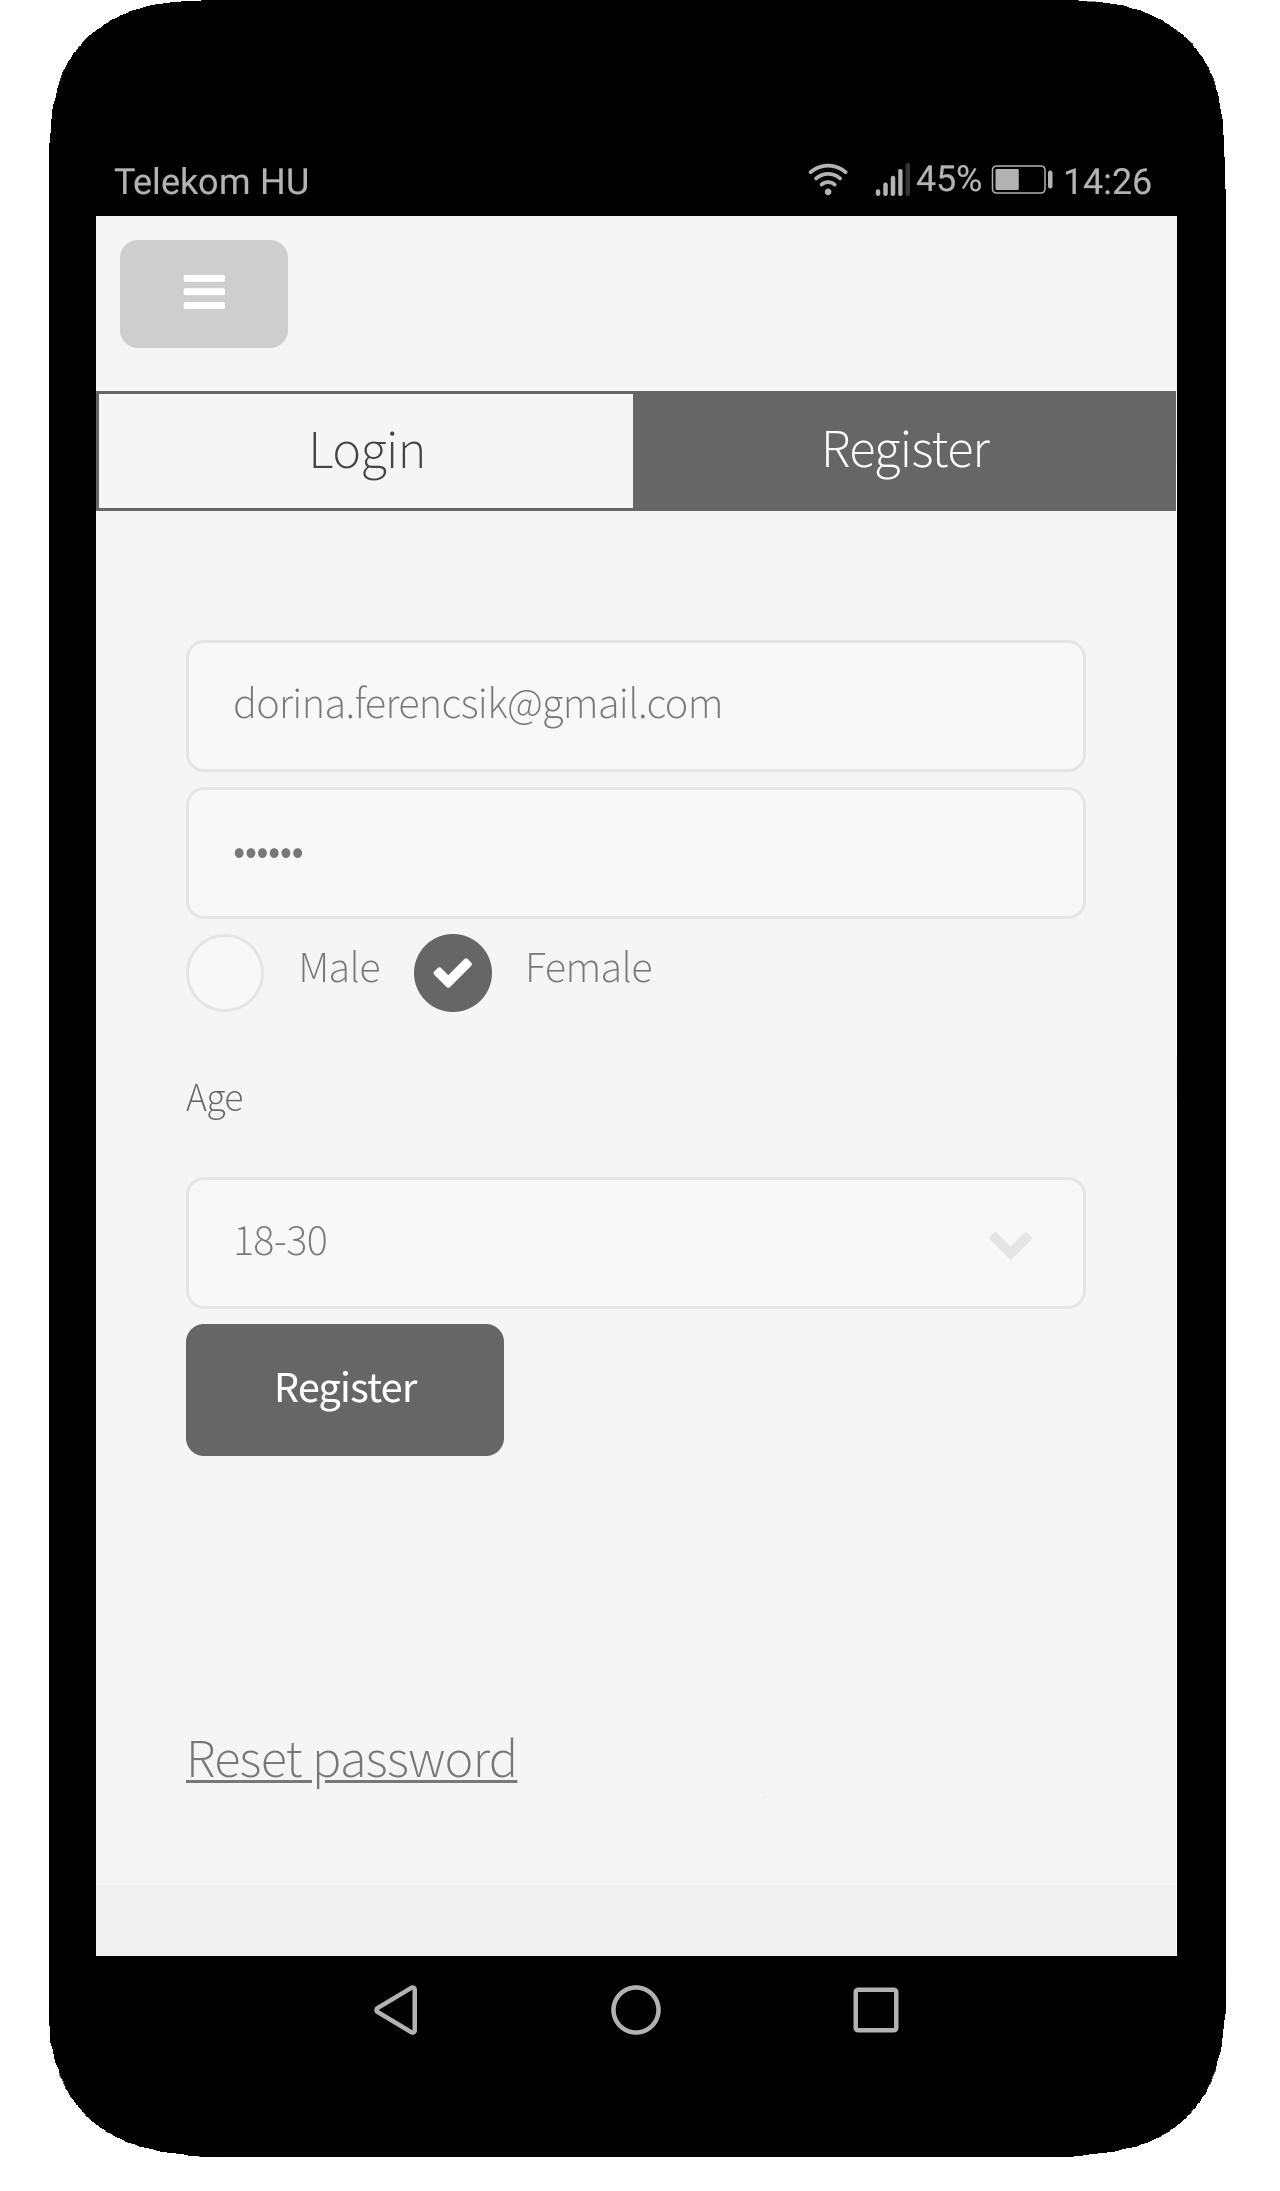
\includegraphics[ width=\textwidth,keepaspectratio]{kepek/website/websiteRegister.png}
		\caption{Regisztráció}
		\label{fig:websiteRegister}
	\end{subfigure}
	\begin{subfigure}[b]{0.35\textwidth}
		\centering
		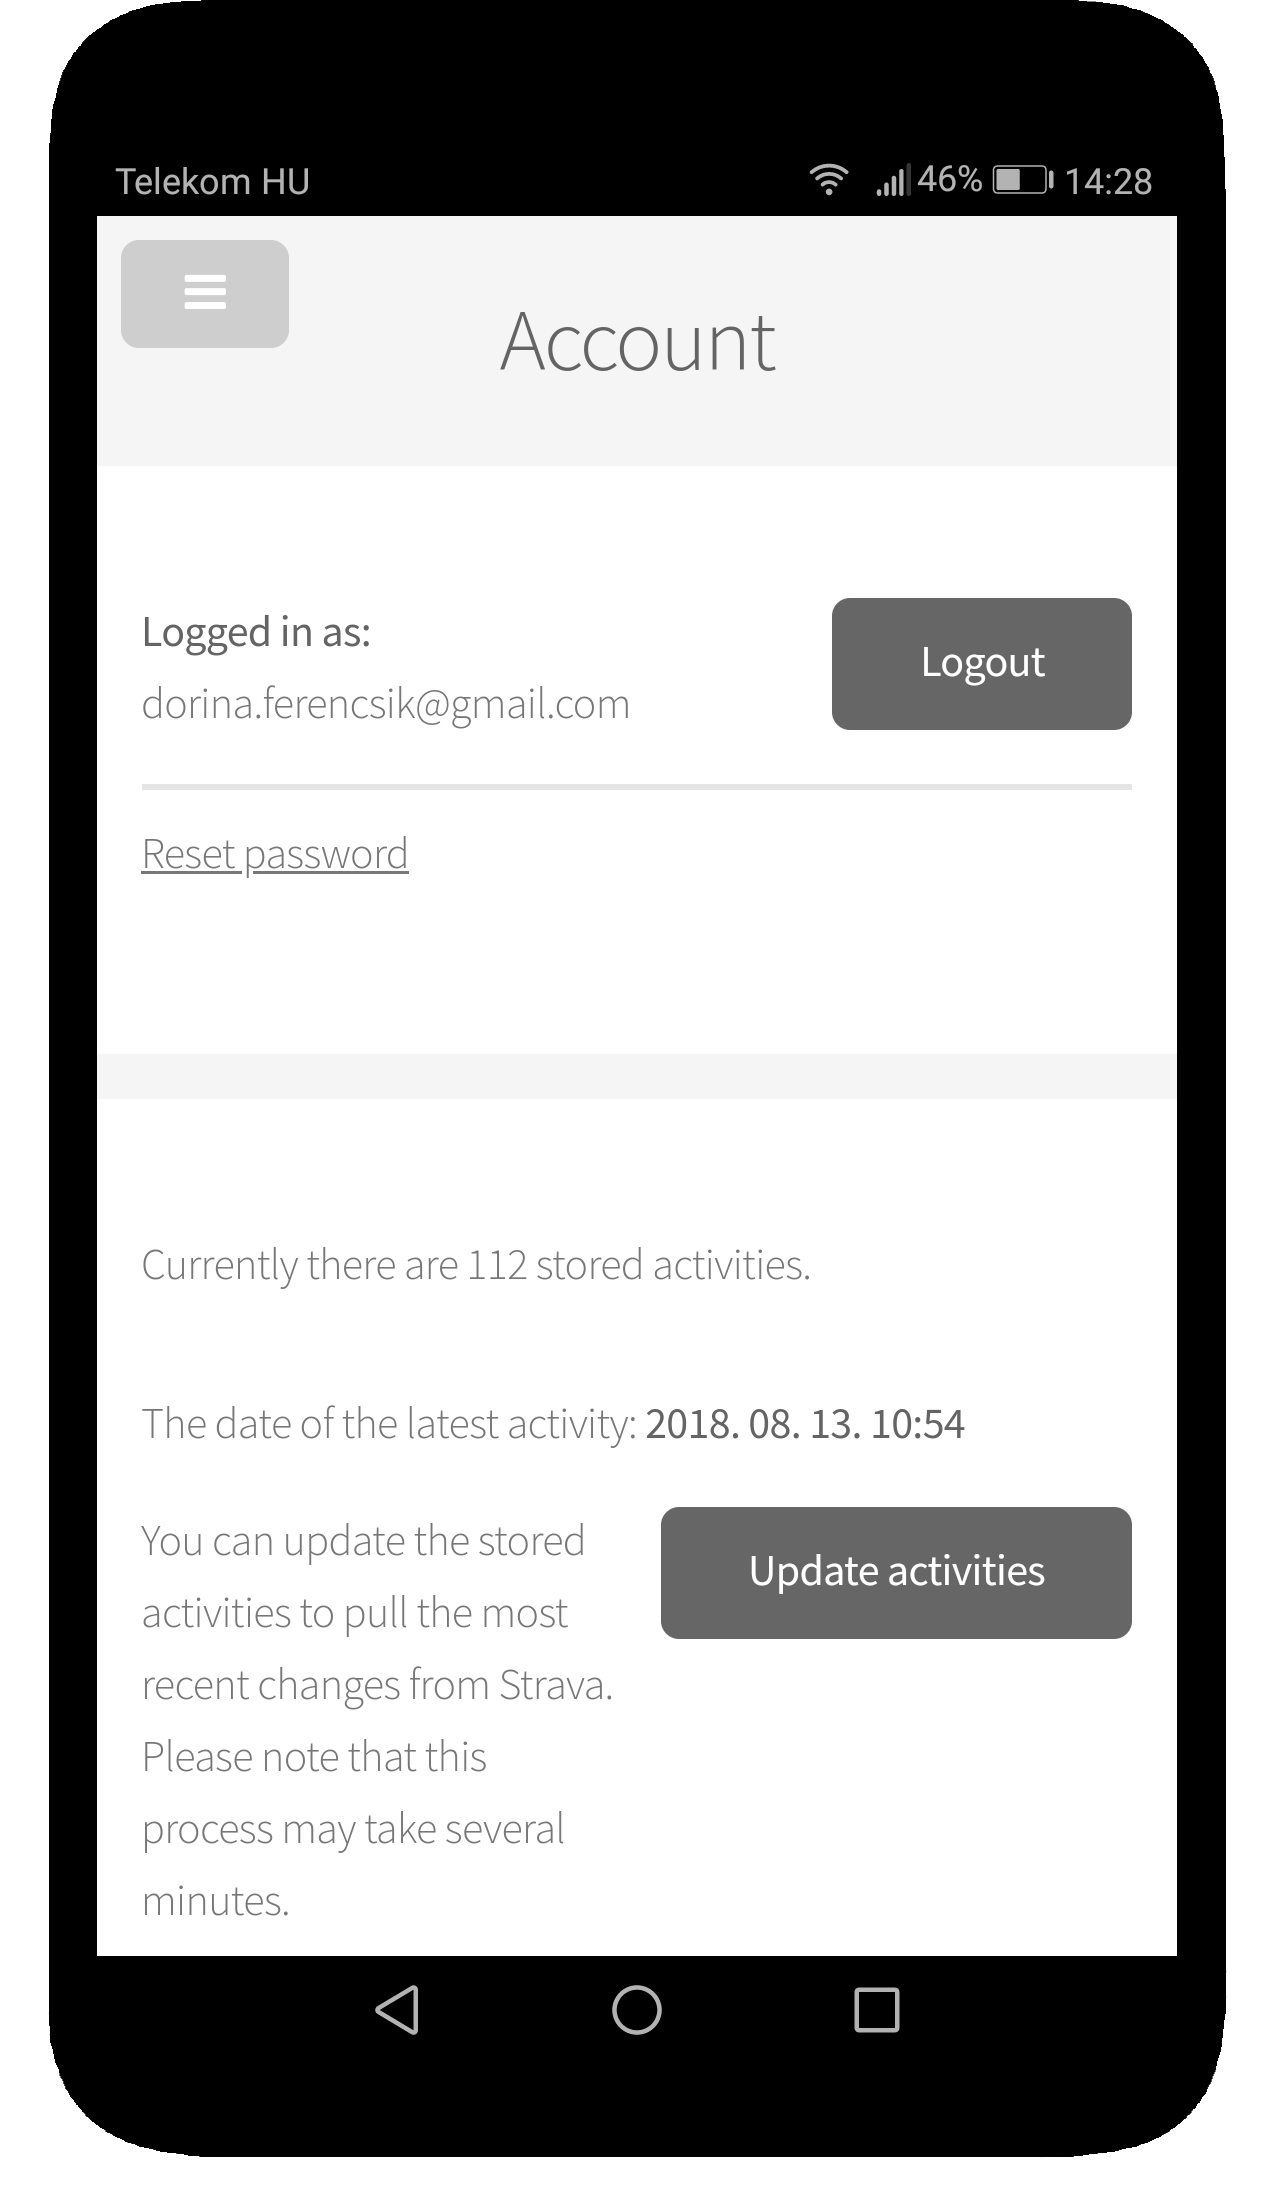
\includegraphics[ width=\textwidth,keepaspectratio]{kepek/website/websiteAccount.png}
		\caption{Fiók}
		\label{fig:websiteAccount}
	\end{subfigure}
	
	\caption{Adatgyűjtő weboldal alapvető funkciói}
%	\label{fig:websiteRegister}
\end{figure}

\subsubsection{JQuery}
A JQuery \cite{jquery} egy népszerű JavaScript könyvtár amely lehetőséget ad a HTML elemek könnyebb manipulálására, az események egyszerűbb kezelésére, animációk megvalósítására. 

\subsubsection{Firebase}
A Firebase \cite{firebase} egy Google által fejlesztett sokoldalú rendszer, amely egyszerű eszközöket kínál egy weboldal logikai részének felépítéséhez. Nem alkalmas robosztus rendszerek létrehozásához, azonban kisebb projektek menedzseléséhez megfelelő alapot kínál. A projekteket létrehozás után online lehet kezelni és a Firebase funkcióit weboldalakban és mobil alkalmazásokban is (mind Android és iOS) egyszerűen lehet használni. A rendszer alapját egy Node.js szerver és egy JSON alapú adatbázis adja valamint elérhető egy általános célú tárhely tetszőleges file-ok tárolásához. 

\subsubsection{Firebase - Autentikáció}
A szakdolgozathoz készített weboldal szempontjából a Firebase egyik legfontosabb eleme az autentikációs rendszer. A Firebase felületén való engedélyezés után a weboldal kódbázisában gyorsan és biztonságosan megvalósítható az új felhasználók regisztrálása, bejelentkeztetése. Az email alapú regisztráláson túl lehetőség van külső rendszerekkel való autentikációra is mint a Google fiók, Facebook, Github. Továbbá elérhető a már regisztrált felhasználók emailen keresztül történő értesítése is.

\subsubsection{Firebase - Adatbázis}
A Firebase alapvetően ingyenes, emiatt az adatbázisnak vannak méret és sebességbeli korlátjai, azonban megfelelő kiindulási alapot ad. A JSON alapú struktúra megkönnyíti az adatok kliens oldalon történő kezelését valamint egy ilyen méretű alkalmazás esetén egyszerűen karban tartható. Fontos kiemelni az adatbázis hozzáférhetőségének konfigurálási lehetőségét. Lehetőség van az adatbázis egészére vagy a részfákra olvasási és írási beállításokat megadni, amik korlátozhatóak a bejelentkezett felhasználó azonosítója alapján is. Ennek felhasználásával könnyen megvalósítható hogy a rendszer összes felhasználója csak a saját adataihoz férjen hozzá ami fontos adatvédelmi szempont.

\SubSection{Adatstruktúra} \label{ssec:adatstruktura}
A szakdolgozathoz készített weboldal fő célja hogy lekérje és tárolja azon felhasználók útvonalait akik regisztrálás után kapcsolódtak a Strava fiókjukhoz. A Strava API-ja az utak lekérésekor SummaryActivity objektumok tömbjével tér vissza, ahol minden objektum 39 változóval jellemez egy utat, aktivitást. Ez a 39 jellemző magába foglalja többek között a felhasználó azonosítóját, a megtett távot, a teljesített kihívások számát, az ismerősök megjegyzéseinek a számát és rengeteg egyéb információt. A gépi tanulás során ezeknek a jellemzőknek csak egy részét érdemes használni, amik szorosabban kapcsolódnak az út valós leírásához. Ezek a jellemzők valamit a felhasználókhoz kapcsolódó adatok szerkezete a \myref{fig:dataStructure} ábrán látható, leírásuk a következőkben kerül részletezésre.

\begin{figure}[!h]
	\centering
	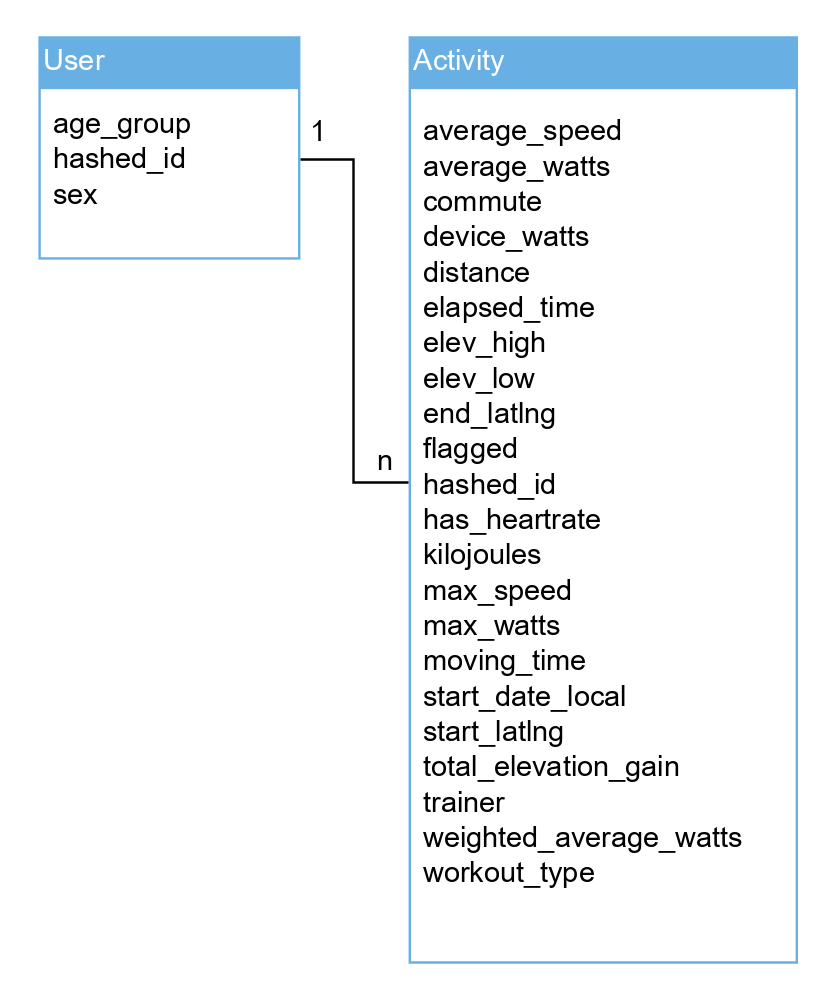
\includegraphics[ width=0.7\textwidth,keepaspectratio]{kepek/data_structure.png}
	\caption{Adatstruktúra}
	\label{fig:dataStructure}
\end{figure}

\noindent \textbf{Jellemzők magyarázata:}
\begin{itemize}
	\item \textbf{age\_group: } felhasználó korcsoportja (0: 18-30; 1: 31-45; 2: 45+)
	\item \textbf{hashed\_id:} felhasználó azonosító hash-elt változata
	\item \textbf{sex: } felhasználó neme (male / female, férfi / nő)
	\item \textbf{average\_speed:} átlagsebesség (méter/másodperc)
	\item \textbf{average\_watts:} átlagos erőkifejtés az útvonal során. Amennyiben nem biztosított az értéke -1
	\item \textbf{commute:} egy tevékenység rögzítésekor lehetőség van azt 'ingázásként' felcímkézni, ezzel megjelölve hogy nem egy verseny vagy túra adat, hanem mindennapi, például munkába vagy boltba járási útvonal. Feltételezhető hogy ilyenkor az illető nem a minél jobb eredmények elérésére törekszik, inkább rutin szerűen, átlagos tempóban halad (logikai; -1 amennyiben nem biztosított)
	\item \textbf{device\_watts:} azt jelöli hogy az erőkifejtési adatokat tényleges mérőkészülék szolgáltatja vagy csupán becsült érték (logikai; Hamis amennyiben becsült érték) 
	\item \textbf{distance:} a megtett távolság (méter)
	\item \textbf{elapsed\_time:} összesen eltelt idő (másodperc)
	\item \textbf{elev\_high:} az út legmagasabb pontja (méter)
	\item \textbf{elev\_low:} az út legalacsonyabb pontja (méter)
	\item \textbf{end\_latlng:} az útvonal végpontjának hosszúsági és szélességi helyzete
	\item \textbf{flagged:} az útvonal meg van e jelölve (logikai)
	\item \textbf{has\_heartrate:} elérhető e pulzus adat (logikai)
	\item \textbf{kilojoules:} összes kifejtett erő mennyisége (kilojoule)
	\item \textbf{max\_speed:} maximum sebesség az út során (méter/másodperc)
	\item \textbf{max\_watts:} maximális erőkifejtés az út során
	\item \textbf{moving\_time:} mozgással töltött idő (másodperc)
	\item \textbf{start\_date\_local:} az út kezdési ideje (dátum)
	\item \textbf{start\_latlng:} az útvonal kezdőpontjának hosszúsági és szélességi helyzete
	\item \textbf{total\_elevation\_gain:} összesen megtett emelkedő (méter)
	\item \textbf{trainer:} az útvonal gépen lett e megtéve (logikai)
	\item \textbf{weighted\_average\_watts:} súlyozott átlagos erőkifejtés az útvonal során. Ha  nem biztosított az értéke: -1.
	\item \textbf{workout\_type:} tevékenység típusa, lehet edzés vagy verseny (egész szám, ha nincs megadva akkor -1. Lehetséges értékei: 10 - normál kerékpározás; 11 - verseny; 12 - edzés )
\end{itemize}










